\documentclass[12pt,a4paper]{article}

% Quelques options d'encodage, de langues et de format du document
\usepackage[utf8]{inputenc}
\usepackage[T1]{fontenc}
\usepackage[english]{babel}
\usepackage[top=2cm, bottom=3cm, left=1.75cm, right=1.75cm]{geometry}
\usepackage{setspace}

\usepackage{graphicx} % Pour la commande "\includegraphics"
\usepackage[ % Modified parameters
    bookmarks,
    colorlinks,
    citecolor=black,
    urlcolor=blue,
    linkcolor=black,
    pdfpagemode=UseNone
]{hyperref} % Pour la commande "\url"

\pagenumbering{arabic}

% ------------------------------------------------------------------
% CITATION MANAGEMENT
% ------------------------------------------------------------------

% APA Style
\usepackage{cite}
%\bibliographystyle{apalike}
\bibliographystyle{ieeetr}

\renewcommand\refname{Bibliography}

% Proper formatting and line breaking for URLs
\usepackage{url}

% Change "References" to "Bibliography"
\usepackage{etoolbox}
\patchcmd{\thebibliography}{\section*{\refname}}{\section*{Bibliography}}{}{}

% ------------------------------------------------------------------
% SUBFIGURE MANAGEMENT
% ------------------------------------------------------------------

\usepackage[caption=false]{subfig}
\usepackage{pgfplots}
\usepgfplotslibrary{groupplots}
\pgfplotsset{compat=1.18}
\usepackage{booktabs}

% ------------------------------------------------------------------
% COLORED TEXT MANAGEMENT
% ------------------------------------------------------------------

\usepackage{todonotes}
\setuptodonotes{inline=always}
\setlength {\marginparwidth }{2cm}
\usepackage{xspace}
\usepackage{amsmath}
\usepackage{cleveref}
\usepackage{multirow}
\usepackage{colortbl}
\usepackage{xcolor}

% needs sheel escape activated
% --shell-escape
%\usetikzlibrary{external}
%\tikzexternalize[prefix=figures_tikz_compiled/]

\definecolor{light-gray}{gray}{0.9}

\usepackage{amsfonts}
\newcommand{\modelministral}{Ministral-8B\xspace}
\newcommand{\modelalpaca}{Alpaca-7B\xspace}
\newcommand{\modeldeepseek}{R1-Distill-8B\xspace}


\begin{document}

\begin{center}
    \begin{tabular}{|p{0.2\textwidth}|p{0.75\textwidth}|}
        \hline
        {
            \vspace{0cm} % without it, bugs, don't know why?
            \centerline{
\includegraphics[width=\linewidth]{./images/tp-ipp}}
        }
        & {
            \vspace{0cm} % same here
            \centering
            \large
            {\hfill February, 2025}

            \vspace*{.5cm}
            \textbf{APM\_5AI29\_TP}

            \vspace*{.5cm}
            \setstretch{1.5}
            {\Large\textbf{Language Models and Structured Data}}

            \vspace*{.5cm}
            Final Project Report

            \vspace*{1cm}
        } \\
        \hline
    \end{tabular}
\end{center}

\noindent Acronym of the Team: AWESome\\
Names: Mochamad Ardiansyah Nurgaha; William Liaw; Eddie Groh; Sriraam Appakutti Palani

    {\centering\rule{\linewidth}{.5pt}}

\begin{center}
    \section*{Knowledge Graph Completion}
\end{center}

% ---------------------------------------------------------
%
% Abstract
%
% ---------------------------------------------------------


\section{Abstract}

This work explores Knowledge Graph Completion (KGC) using two similar approaches: prompt-based tail entity ranking and fine-tuning-based triple classification.
By leveraging structured retrieval for ranking candidates and integrating knowledge-infused prompts for classification, we assess the effectiveness of different large language models across various KGC tasks.

% ---------------------------------------------------------
%
% PROBLEM STATEMENT
%
% ---------------------------------------------------------


\section{Problem Statement}\label{sec:problem-statement}

Knowledge Graph Completion aims to infer missing facts in a knowledge graph (KG) by leveraging existing structural and semantic relationships.
A knowledge graph consists of entities, relations, and triples of the form \( (h, r, t) \), where \( h \) (head) and \( t \) (tail) are connected by relation \( r \).
Due to the inherent incompleteness of KGs, KGC seeks to either predict missing entities or verify candidate triples.

Although KGC is often framed as a single task, different methodological approaches necessitate distinct problem formulations.
In this work, we focus on two complementary tasks: \emph{link prediction} and \emph{triple classification}.
This distinction reflects the differences in the evaluated approaches.
While it is certainly possible to adapt both approaches to a unified setting, doing so would require significant modifications that could change their original design.
To preserve the intended methodology from the papers, we therefore opted to maintain these two slightly different problem formulations.

\paragraph{Link Prediction:}
Link prediction involves inferring a missing entity in an incomplete triple. Given \( (h, r, ?) \) or \( (?, r, t) \), the goal is to rank candidate entities based on their plausibility as a valid completion.

\paragraph{Triple Classification:}
Triple classification assesses whether a given triple \( (h, r, t) \) is valid. Instead of ranking candidates, the model outputs a binary decision indicating whether the relationship holds.

% ---------------------------------------------------------
%
% BACKGROUND
%
% ---------------------------------------------------------


\section{Background}\label{sec:background}

Early KGC research centered on triple-based models using embedding methods to represent entities and relations in a continuous vector space.
TransE~\cite{bordes2013translating} models relations as translation operations, while DistMult~\cite{yang2014embedding} and ComplEx~\cite{trouillon2016complex} apply tensor factorization, the latter extending to complex-valued embeddings.

%Advancements introduced Graph Neural Networks (GNNs)~\cite{schlichtkrull2018modeling} to refine entity representations by aggregating structural information.
%However, these models struggle with long-tail entities due to sparse connectivity, limiting predictive performance.

%To overcome these limitations, text-based KGC leverages pre-trained language models (PLMs) to incorporate entity and relation descriptions. KG-BERT~\cite{yao2019kgbert} reframes KGC as a classification problem, encoding triples as text for distinguishing valid from invalid ones.
%Despite effectiveness, these methods require extensive fine-tuning and high computational costs, restricting scalability.

Large Language Models (LLMs) have revolutionized KGC by leveraging their broad internal knowledge and advanced reasoning capabilities.
This enables, in some cases, the ability to perform link prediction without even being trained on the target data, using techniques such as in-context learning and instruction tuning.
Unlike traditional KG models, which rely on structured embeddings, LLMs offer greater flexibility for zero-shot and few-shot predictions.
However, they often struggle with hallucination and structural misalignment with KG schemas.


We divide LLM-based KGC solutions into two main categories:

\paragraph{Purely Prompt-Based Methods:} These exploit structured retrieval or textual descriptions alongside in-context learning, without modifying LLM parameters.
For instance, MPIKGC~\cite{xu2024mpikgc} enhances description-based KGC models by querying LLMs to expand entity representations, thereby improving relation understanding and capturing structural clues.
KICGPT~\cite{wei2023kicgpt} stands out by incorporating a triple-based retriever for preliminary ranking, then refining the candidate list through \emph{Knowledge Prompts} that encode KG structure directly into the LLM's prompts.
Although KICGPT's approach remains parameter-free, it injects structural awareness more explicitly than simpler prompt-based methods.

\paragraph{Fine-Tuning-Based Methods:} These methods embed KG structure into the LLM through additional training.
For example, DIFT~\cite{liu2024dift} refines the model with discrimination instructions to better identify valid entities, while KC-GenRe~\cite{wang2024kcgenre} adopts a knowledge-constrained re-ranking technique, updating LLM weights to emphasize entity ranking.
%RPKGC~\cite{khalil2024rpkgc} fine-tunes a model for relation prediction, learning to infer plausible connections between entity pairs.
Finally, KoPA~\cite{qin2023kopa} integrates a \emph{Knowledge Prefix Adapter}, mapping KG embeddings into the LLM's textual space to guide inference with structural signals.
Although KoPA modifies model weights, it keeps the KG structure directly accessible during generation and prediction.


% ---------------------------------------------------------
%
% METHODOLOGY
%
% ---------------------------------------------------------


\section{Methodology}\label{sec:methodology}

Following the analysis in \cref{sec:background}, we now outline our methodological approach to KGC. Our work examines one representative method from each of the previously discussed categories: KICGPT, a purely prompt-based approach for tail prediction, and KoPA, which applies fine-tuning for triple classification.

\subsection{KICGPT: Prompt-Based Link Prediction}
\label{sec:method:kicgpt}

\begin{figure}
    \centering
    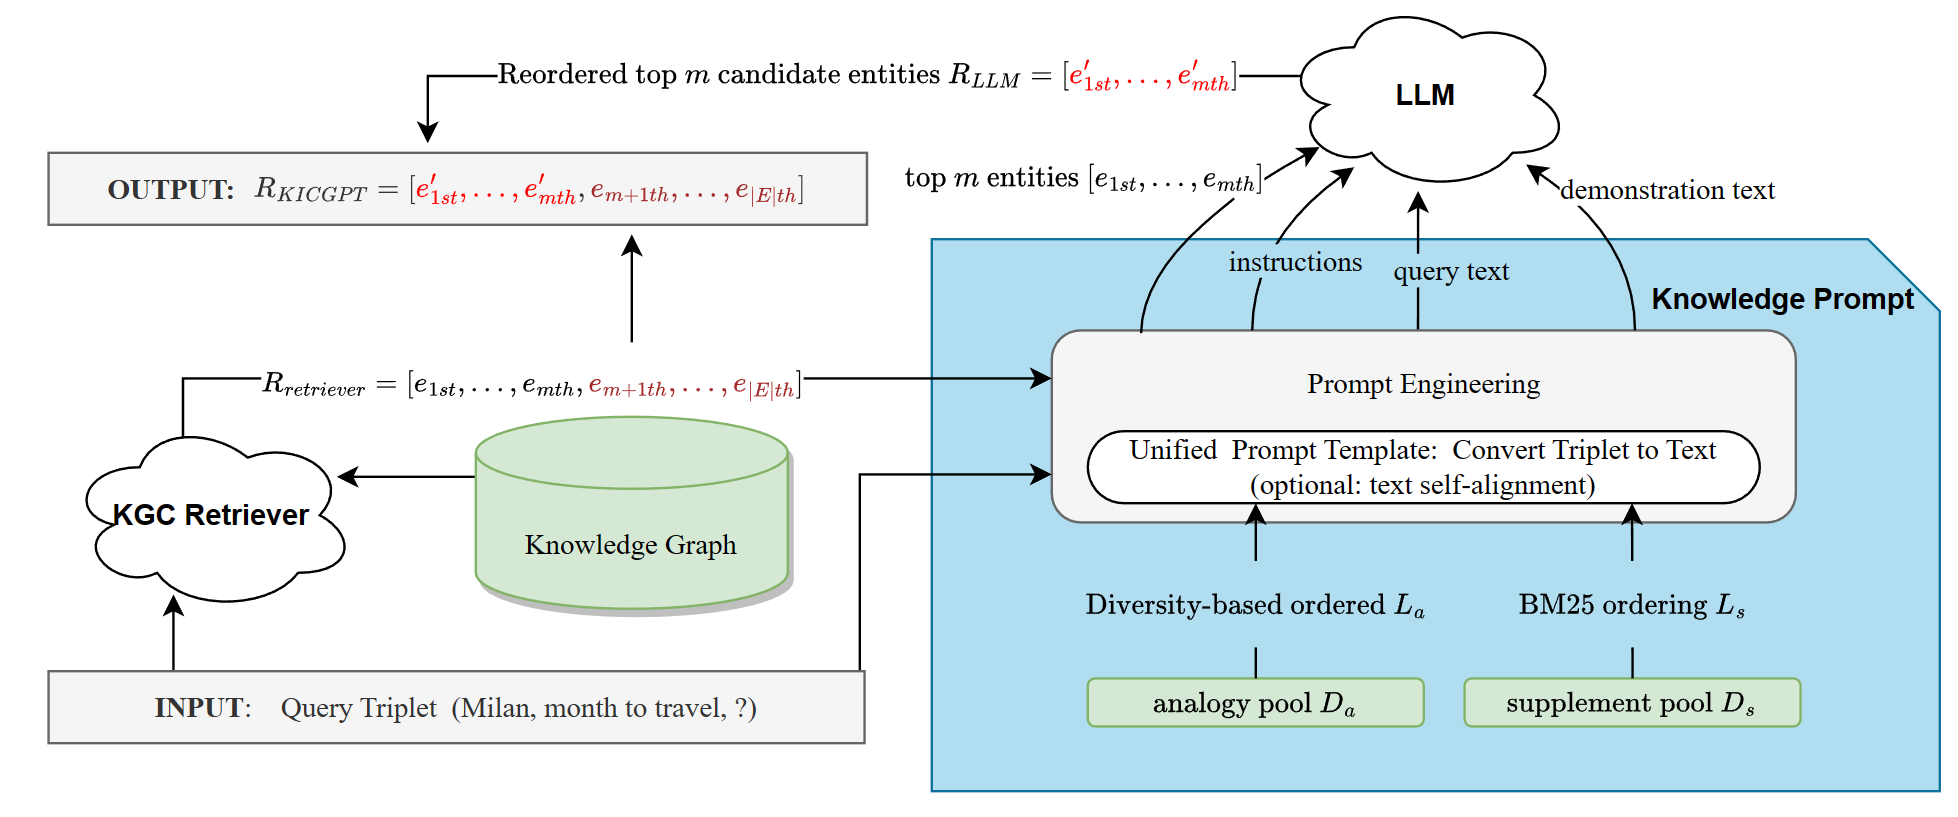
\includegraphics[width=0.99\textwidth]{figures/KICGPTarchitecture}
    \caption{KICGPT architecture, consisting of a triple-based KGC retriever, the \emph{Knowledge Prompt}, and an LLM-based reranker \cite{wei2023kicgpt}.}
    \label{fig:KICGPTarchitecture}
\end{figure}

KICGPT primarily consists of three components, as illustrated in \cref{fig:KICGPTarchitecture}: a triple-based KGC retriever, a \emph{Knowledge Prompt} module, and an LLM-based reranker.
Given a query triple \( (h, r, ?) \) from a KG \(G\) consisting of set of entities \(E\) and relations \(R\), the retriever computes a ranking over all possible entities \( e \in E \), generating an initial ordered list \( R_{\text{retriever}} = [e_1, e_2, ..., e_{|E|}] \) based on a predefined scoring function. The \emph{Knowledge Prompt} then provides structured in-context learning examples to guide the LLM, which subsequently refines the top-\( m \) candidates, producing a reranked list \( R_{\text{LLM}} = [e'_1, e'_2, ..., e'_m] \).
The final output of KICGPT combines the LLM’s refined ranking with the remaining entities from the retriever, yielding the final entity ranking:

\[
    R_{\text{KICGPT}} = [e'_1, e'_2, ..., e'_m, e_{m+1}, ..., e_{|E|}].
\]

\subsubsection{Knowledge Prompt Construction}

The \emph{Knowledge Prompt} enables KICGPT to leverage in-context learning by integrating relevant KG information into the LLM’s input.
The prompt is constructed from two pools of triples: the analogy pool \( D_a \) and the supplement pool \( D_s \).
The analogy pool consists of triples that share the same relation \( r \) as the query, ensuring that the LLM is exposed to examples with similar relational structures:

\[
    D_a = \{(e', r, e'') \in G \mid e', e'' \in E\}.
\]

The supplement pool contains triples where the head or tail entity matches the query's head entity \( h \), providing additional entity-specific context:

\[
    D_s = \{(h, r', e') \in G \mid r' \in R, e' \in E\} \cup \{(e', r', h) \in G \mid r' \in R, e' \in E\}.
\]

To ensure that the most relevant demonstrations are selected, triples in \( D_s \) are ranked using BM25 scores, which measure textual similarity to the query entity description.
The final ordered sets, denoted as \( L_a \) for analogy-based examples and \( L_s \) for supplement-based examples, are constructed to optimize the informativeness of the prompt.
For the analogy pool, entity counters are initialized at zero, and triples are iteratively selected to maximize diversity while minimizing repetition.

\subsubsection{Prompt Engineering and Query Processing}

To effectively incorporate the selected examples, KICGPT transforms structured triples into natural language statements using a unified prompt template.
This ensures consistent formatting across queries and demonstrations, making the input more interpretable for the LLM. The prompt follows a structured process consisting of the following phases:

\begin{itemize}
    \item \textbf{Task Description:} The prompt begins with a responsibility statement that explicitly clarifies the LLM’s role in ranking candidate entities based on relational context.
    \item \textbf{Query Introduction:} The incomplete triple \( (h, r, ?) \) is presented, ensuring the model understands the missing component it must predict.
    \item \textbf{Demonstration Explanation:} The two sources of contextual examples, analogy-based triples \( L_a \) and supplement-based triples \( L_s \), are described so that the LLM can recognize their significance in guiding predictions.
    \item \textbf{Demonstration Integration:} Selected triples from \( L_a \) and \( L_s \) are appended to the prompt.
    The number of demonstrations is maximized within the LLM’s token limit to provide sufficient context.
    \item \textbf{Re-Ranking and Final Prediction:} The LLM processes the structured prompt and re-ranks the top-\( m \) candidates, producing an ordered list \( R_{\text{LLM}} \).
    The highest-ranked entities from this list replace the corresponding top-\( m \) results from the retriever, yielding the final ranking.
\end{itemize}

\subsection{KoPA: Fine-Tuning-Based Triple Classification}

\begin{figure}
    \centering
    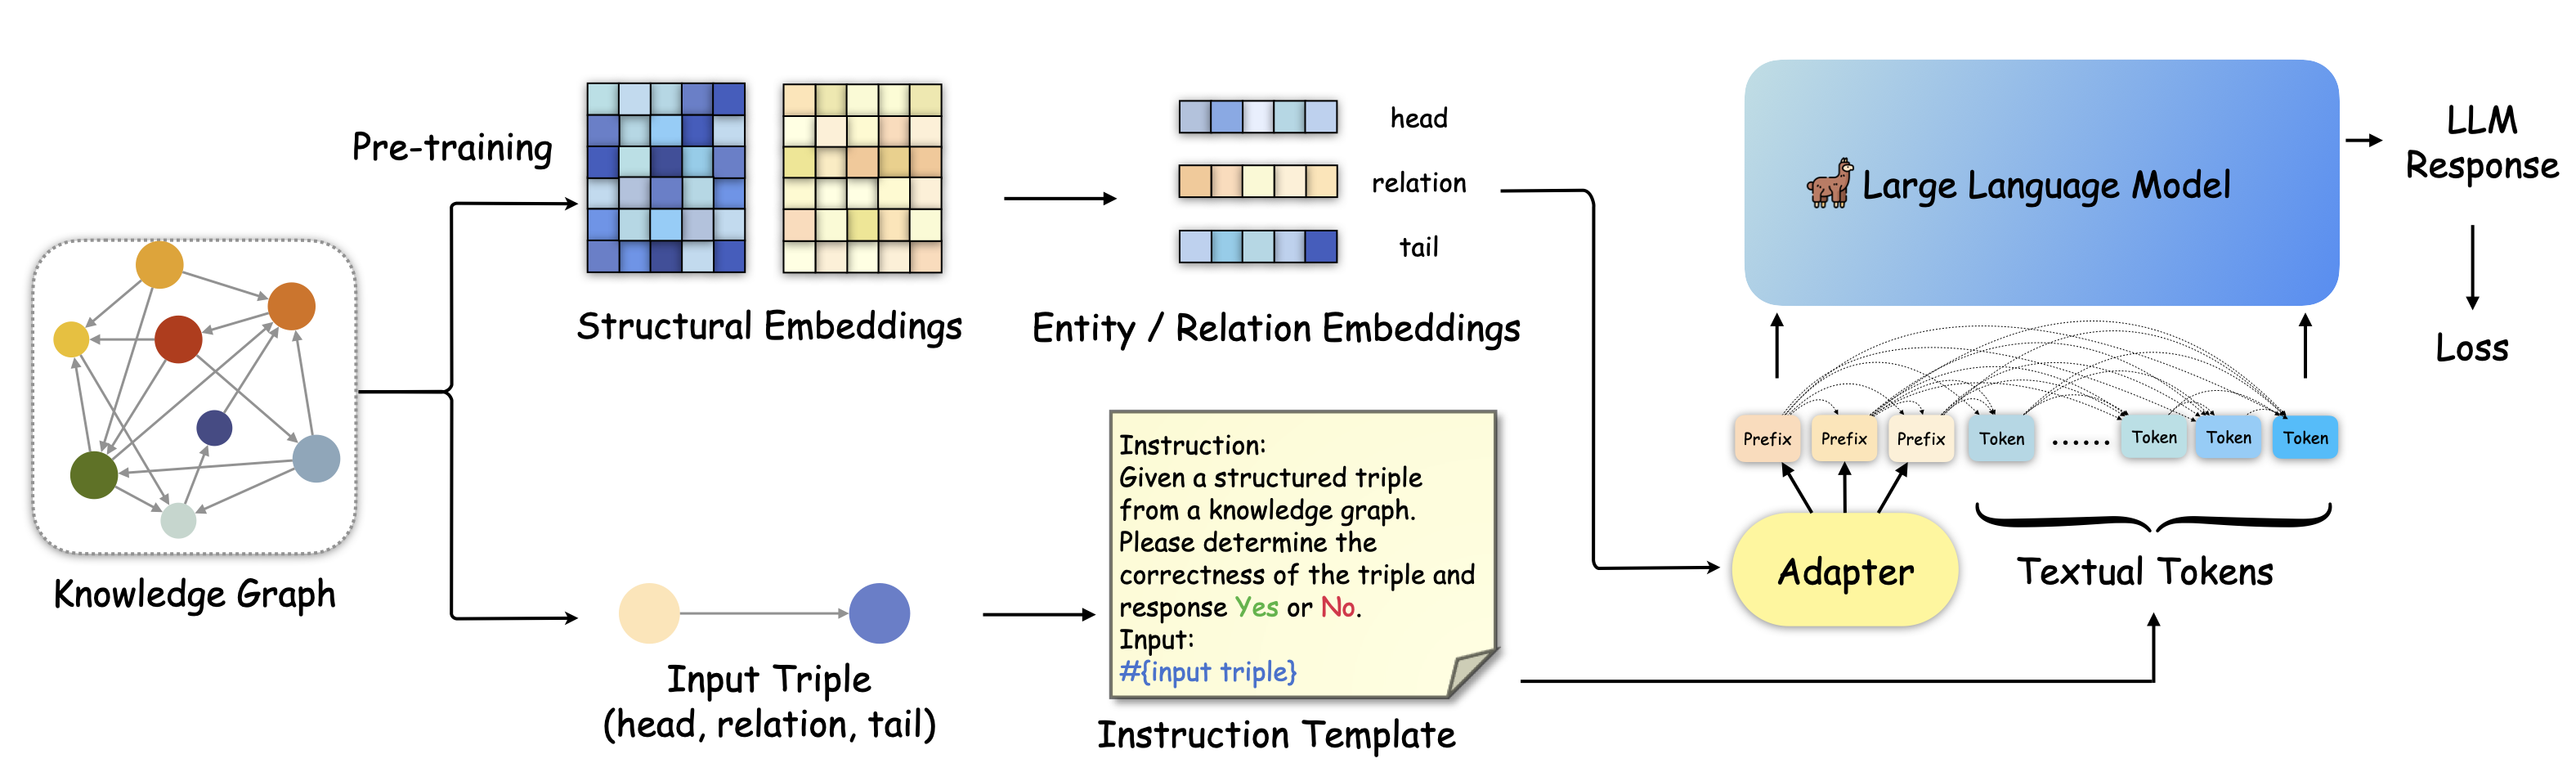
\includegraphics[width=0.99\textwidth]{figures/KoPAarchitecture}
    \caption{KoPA architecture: Entities and relations are converted into empeddings, which after adaptation can then be incooperated directly into the LLM \cite{qin2023kopa}.}
    \label{fig:KoPAarchitecture}
\end{figure}

KoPA addresses the triple classification problem by embedding structured knowledge graph representations into the LLM’s reasoning process, explicitly incorporating KG structure through fine-tuning rather than relying on prompt-based ranking.
By leveraging structured KG embeddings, KoPA enhances the LLM’s ability to distinguish between valid and invalid triples, integrating relational constraints directly into its decision-making process.
As illustrated in \cref{fig:KoPAarchitecture}, the model combines structural embeddings with a knowledge prefix adapter, enabling a seamless fusion of KG-based constraints with LLM inference.

\subsubsection{Structural Embeddings}
To integrate KG structure, each entity \( e \) and relation \( r \) is mapped into a latent vector space, where relational dependencies are preserved.
The learned embeddings, denoted as \( \mathbf{e} \in \mathbb{R}^{d_e} \) for entities and \( \mathbf{r} \in \mathbb{R}^{d_r} \) for relations, capture topological and semantic information from the KG. A scoring function \( F(h, r, t) = \mathbf{h}^\top \mathbf{W_r} \mathbf{t} \), where \( \mathbf{h}, \mathbf{t} \) are entity embeddings and \( \mathbf{W_r} \) is a relation-specific transformation matrix, is used to estimate the plausibility of a triple.

These embeddings are pre-trained using self-supervised learning, ensuring that relational constraints are reflected in the representation space.
Unlike textual descriptions, which can be noisy or incomplete, structured embeddings provide a more direct way of modeling entity relationships.
By aligning embeddings with the LLM’s input, KoPA ensures that structural information is explicitly available during inference.

\subsubsection{Knowledge Prefix Adapter}

To bridge structured embeddings with the LLM’s textual processing, KoPA employs a \textit{Knowledge Prefix Adapter} (KPA).
This adapter transforms structured embeddings into a virtual prefix, effectively mapping entity and relation representations into the model’s input space. Given a triple \( (h, r, t) \), the adapter projects its corresponding embeddings \( \mathbf{h}, \mathbf{r}, \mathbf{t} \) into a sequence of virtual tokens, denoted as \( K = P(\mathbf{h}) \oplus P(\mathbf{r}) \oplus P(\mathbf{t}) \), where \( P \) is a learned transformation function.

The knowledge prefix is prepended to the LLM’s textual input, allowing the model to condition its predictions on structured KG information.
This approach ensures that the model retains relational constraints while maintaining flexibility in handling natural language inputs.
Unlike fully fine-tuned KG embeddings, which modify the LLM’s internal parameters, the prefix adapter enables lightweight structural integration without overfitting to specific KG schemas.

\subsubsection{Fine-Tuning and Classification}
% KoPA is trained on a dataset of valid and invalid triples to optimize its ability to distinguish factual from incorrect knowledge.
% Given an input triple \( (h, r, t) \), the model computes a classification score \( g(h, r, t) \), indicating the likelihood that the triple is valid.
% The knowledge prefix adapter ensures that the LLM considers both explicit KG structure and learned textual reasoning when making classification decisions.
% This hybrid approach leverages the strengths of structured embeddings while retaining the adaptability of large-scale LLMs.

The knowledge prefix and the textual input are jointly processed by the LLM,
which predicts the validity of the input triple based on the combined information.
The LLM is fine-tuned on the instruction-following task to optimize its triple classification accuracy.
% ---------------------------------------------------------
%
% EXPERIMENTS
%
% ---------------------------------------------------------


\section{Experiments}\label{sec:experiments}

\subsection{Datasets}

For our experiments, we used two widely adopted KGC benchmarks, which are summarized in \cref{tab:datasets}.

\paragraph{WN18RR} is a filtered version of WN18~\cite{wn18rr}, derived from WordNet~\cite{wordnet}, designed to eliminate inverse relations that previously made link prediction trivial.
This refinement increases task difficulty, requiring models to generalize beyond simple pattern recognition.

\paragraph{CoDeX-S} (Complex Dataset Extracted from Wikidata~\cite{wikidata}) is a subset of CoDeX~\cite{safavi2020codex}, offering a diverse set of relational facts.
Unlike WN18RR, which focuses on lexical semantics, CoDeX-S is sourced from Wikidata, ensuring a richer relational structure with a more balanced distribution of relations.

\begin{table}
    \centering
    \begin{tabular}{l c c c c c}
        \hline
        Dataset & \#Entities & \#Relations & \#Train & \#Test \\
        \hline
        WN18RR  & 40,943     & 11          & 86,835  & 3,134  \\
        CoDeX-S & 2,034      & 42          & 32,888  & 3,654  \\
        \hline
    \end{tabular}
    \caption{Statistics of the datasets used in our experiments.}
    \label{tab:datasets}
\end{table}

\subsection{Language Models}

To evaluate model performance across different architectures, we consider three language models with distinct capabilities:

\paragraph{Alpaca-7B}~\cite{taori2023stanford} is a fine-tuned variant of LLaMA 7B, trained on 52,000 instruction-response pairs generated by OpenAI’s text-davinci-003.
Optimized for general instruction-following, it serves as a lightweight baseline.

\paragraph{Mistral-8B-Instruct-2410}~\cite{mistralai2024ministral8b} is an 8-billion-parameter model designed for instruction-based tasks, featuring a 128k-token context window and multilingual support.
Compared to Alpaca-7B, it benefits from a slightly larger model size, extended context length, and improved cross-lingual capabilities.

\paragraph{DeepSeek-R1-Distill-Llama-8B}~\cite{deepseekai2025deepseekr1distillllama8b} is a distilled version of DeepSeek-R1~\cite{guo2025deepseek}, optimized for reasoning and problem-solving.
With a strong emphasis on mathematical and coding tasks, it is particularly effective in structured problem domains.

\subsection{Evaluation of the KICGPT Approach}

\begin{figure}
    \centering
    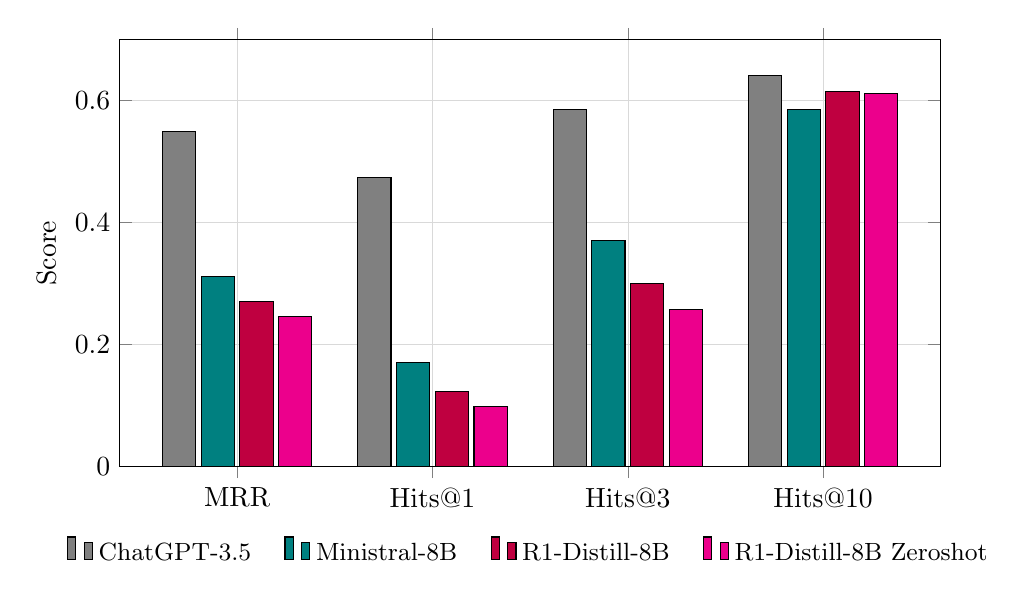
\begin{tikzpicture}
        \begin{axis}[
            ybar, bar width=12pt,
            symbolic x coords={MRR, Hits@1, Hits@3, Hits@10},
            xtick=data, ymin=0, ymax=0.7, ylabel={Score}, width=12cm, height=7cm, grid=both,
            major grid style={line width=.2pt, draw=gray!30},
            minor grid style={draw=gray!10},
            enlarge x limits=0.2,
        % Legend placed below with spacing:
            legend style={
                at={(0.5,-0.15)}, anchor=north,
                /tikz/every even column/.append style={column sep=10pt},
                legend columns=4, draw=none, fill=none, font=\small
            }]
            % Bars
            \addplot[fill=gray]   coordinates {(MRR,0.549)  (Hits@1,0.474)  (Hits@3,0.585)  (Hits@10,0.641)};
            \addlegendentry{ChatGPT-3.5}
            \addplot[fill=teal]   coordinates {(MRR,0.3112) (Hits@1,0.1707) (Hits@3,0.3711) (Hits@10,0.5862)};
            \addlegendentry{\modelministral}
            \addplot[fill=purple] coordinates {(MRR,0.2700) (Hits@1,0.1233) (Hits@3,0.2994) (Hits@10,0.6145)};
            \addlegendentry{\modeldeepseek}
            \addplot[fill=magenta] coordinates {(MRR,0.2461) (Hits@1,0.0980) (Hits@3,0.2580) (Hits@10,0.6120)};
            \addlegendentry{\modeldeepseek Zeroshot}
        \end{axis}
    \end{tikzpicture}
    \caption{Comparison of our results on the WN18RR test set with those from Wei et al.~\cite{wei2023kicgpt} (shown in gray). We evaluated \modelalpaca and \modeldeepseek using the same methodology, but also including a zero-shot setting.
    }
    \label{fig:kicgpt_evaluation_link_ordering}
\end{figure}

\begin{table}
    \centering
    \begin{tabular}{l|l|c|c|c|c}
        \toprule
        \textbf{Model}                   & \textbf{MRR}   & \textbf{Hits@1} & \textbf{Hits@3} & \textbf{Hits@10} \\
        \midrule

        ChatGPT (Theirs)                 & \textbf{0.564} & \textbf{0.478}  & \textbf{0.612}  & \textbf{0.677}   \\
        Mistral-7B (Ours)                & 0.3112         & 0.1707          & 0.3711          & 0.5862           \\
        DeepSeek-7B (Ours)               & 0.2700         & 0.1233          & 0.2994          & 0.6145           \\
        DeepSeek-7B$_{zero-shot}$ (Ours) & 0.2461         & 0.0980          & 0.2580          & 0.6120           \\

        \bottomrule
    \end{tabular}
    \caption{Results from \cref{fig:kicgpt_evaluation_link_ordering} in tabular format. See \cref{tab:kicgpt_detailed_comparison} in appendix for detailled comparison.}
    \label{tab:kicgpt_evaluation_link_ordering}
\end{table}


All experiments were conducted on a system equipped with an NVIDIA RTX A5000 GPU with 24 GiB of VRAM, an Intel Xeon W-1270P CPU running at 3.80 GHz, and 64 GB of RAM.

As previously discussed, this approach does not require modifications to the models themselves.
However, while the original implementation relied on the ChatGPT API, we adapted it to locally running models.
Specifically, in \cref{fig:kicgpt_evaluation_link_ordering} we evaluated \modelministral and \modeldeepseek, comparing their performance against the results reported by Wei et al.~\cite{wei2023kicgpt}.

\modelministral followed prompt instructions closely and rarely produced unparsable output.
However, it significantly underperformed compared to the original study,
which we tentatively attribute to ChatGPT-3.5’s superior general knowledge and reasoning capabilities.

\modeldeepseek demonstrated strong reasoning abilities inside its explicit thinking tags, effectively analyzing given options, recognizing patterns, and identifying preferable choices.
However, this process was often excessively verbose, even when explicitly instructed to be concise.
Additionally, it frequently truncated its final responses, replacing parts of the output with ellipses (\dots), likely due to a focus loss while reasoning about the problem.
Moreover, \modeldeepseek sometimes disregarded specific prompt instructions, potentially because it is primarily tuned for mathematical and coding tasks.
Since the full-size Deepseek-R1 model is known to suffer from degraded performance with few-shot prompting~\cite{guo2025deepseek}, a similar issue may affect this distilled variant.
However, as the few-shot examples contain domain-specific information, removing them entirely could also further reduce performance.

Both models performed surprisingly on-par with ChatGPT in the Hits@10 evaluation.
However, this is likely due to variations in output length rather than genuine ranking improvements.
Since evaluation is based on the options generated by the LLM rather than the full ground-truth ranking, models that produce shorter responses inherently increase their chances of including the correct answer among the top-ranked candidates.

\subsection{Evaluation of the KoPA Approach}

\begin{figure}
    \centering
    \begin{tikzpicture}
        % Group plot configuration
        \begin{groupplot}[
            group style={
                group size=3 by 1,       % 3 plots in 1 row
                horizontal sep=0.3cm     % Adjust spacing between plots
            },
            width=0.38\textwidth,        % Maximized plot width
            ymode=log,                   % Log-scale y-axis for ALL plots
            xmin=0, xmax=3,              % Unified x-axis range
            ymin=1e-3, ymax=1,           % Unified y-axis range across all plots
            xlabel=Epoch,
            xtick distance=0.5,          % Uniform tick spacing
            ytick distance=10,           % Log-scale tick separation
            minor y tick num=9,          % Minor tick marks for readability
        ]

            %------------- Plot (a) Alpaca -----------------
            \nextgroupplot[
                title=\modelalpaca,
            % Hide y-axis labels for alignment
                ylabel=Loss / Gradient Norm
            ]
            \addplot[smooth, thick, blue]
            table[x=epoch, y=loss, col sep=space]
                {figures/raw-data/lora-Llama-2-7b-alpaca-cleaned-finetune.dat};

            \addplot[smooth, thick, cyan, dashed]
            table[x=epoch, y=grad-norm, col sep=space]
                {figures/raw-data/lora-Llama-2-7b-alpaca-cleaned-finetune.dat};


            %------------- Plot (b) DeepSeek ---------------
            \nextgroupplot[
                title=\modeldeepseek,
                yticklabels={,,}
            ]
            \addplot[smooth, thick, purple]
            table[x=epoch, y=loss, col sep=space]
                {figures/raw-data/lora-DeepSeek-R1-Distill-Llama-8B-finetune.dat};

            \addplot[smooth, thick, violet, dashed]
            table[x=epoch, y=grad-norm, col sep=space]
                {figures/raw-data/lora-DeepSeek-R1-Distill-Llama-8B-finetune.dat};

            %------------- Plot (c) Loss Comparison -------------
            \nextgroupplot[
                title=Loss Comparison,
                yticklabels={,,}   % Hide y-axis tick labels for uniform look
            ]
            \addplot[smooth, thick, purple]
            table[x=epoch, y=loss, col sep=space]
                {figures/raw-data/lora-DeepSeek-R1-Distill-Llama-8B-finetune.dat};

            \addplot[smooth, thick, blue]
            table[x=epoch, y=loss, col sep=space]
                {figures/raw-data/lora-Llama-2-7b-alpaca-cleaned-finetune.dat};

        \end{groupplot}
    \end{tikzpicture}

    % Description of colors with more spacing in legend
    \vspace{0.2cm}
    {\centering
        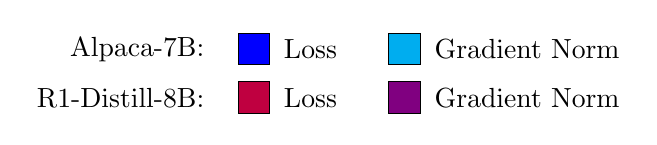
\begin{tikzpicture}
            \node[draw, fill=blue, minimum width=0.4cm, minimum height=0.4cm] (A) {};
            \node[left=0.3cm of A] {\modelalpaca:};
            \node[right=0.05cm of A] {Loss};

            \node[draw, fill=cyan, minimum width=0.4cm, minimum height=0.4cm, right=1.5cm of A] (B) {};
            \node[right=0.05cm of B] {Gradient Norm};

            \node[draw, fill=purple, minimum width=0.4cm, minimum height=0.4cm, below=0.2cm of A] (C) {};
            \node[left=0.3cm of C] {\modeldeepseek:};
            \node[right=0.05cm of C] {Loss};

            \node[draw, fill=violet, minimum width=0.4cm, minimum height=0.4cm, right=1.5cm of C] (D) {};
            \node[right=0.05cm of D] {Gradient Norm};
        \end{tikzpicture}
    }

    \caption{Our fine-tuning process of \modelalpaca and \modeldeepseek on the CoDeX-S dataset. Loss and gradient norm trends are shown separately for each model, along with a comparison of both losses.}
    \label{fig:kopa_finetuning_process}
\end{figure}


Following the procedure outlined in~\cref{sec:methodology}, we fine-tuned \modelalpaca on the CoDeX~\cite{safavi2020codex} dataset.
The process took 10 hours and 12 minutes, with the model converging as expected.
As shown in \cref{fig:kopa_finetuning_process}, the training loss follows a slightly noisy downward trend, while the gradient norm exhibits significant fluctuations but generally decreases over time.

Using the same setup, \modeldeepseek was fine-tuned in 9 hours and 56 minutes.
Its loss curve closely resembles that of \modelalpaca, confirming stable convergence, though the gradient norm remains similarly volatile.
A direct comparison reveals that both models exhibit nearly identical loss trajectories, which would suggest that they should have comparable performance.

We evaluated the prediction performance of \modelalpaca and \modeldeepseek on the CoDeX-S test set and compared our results to those reported by Qin et al.~\cite{qin2023kopa}.
As shown in \cref{fig:codex_kopa_evaluation}, both models achieve similar overall results, with \modeldeepseek consistently lagging slightly behind \modelalpaca across all metrics.
The evaluation process took 52 minutes for \modelalpaca and 56 minutes for \modeldeepseek.

While we follow the same methodological approach as the original work, our results fall significantly short of the reported performance.
The cause of this discrepancy is unclear, though possible explanations include minor differences in hyperparameters such as batch size and learning rate, which we had to adjust to accommodate our computational constraints.
However, given the extent of the performance gap, it is very unlikely that these adjustments alone fully explain the differences.

A notable issue observed in both models is a strong bias toward classifying triples as true.
Despite the test set containing an equal distribution of true and false triples (1828/1828), \modelalpaca classified 3472 triples as true and only 184 as false, while \modeldeepseek classified 3558 as true and only 98 as false.
This skew results in exceptionally high recall, reaching up to 99\% for \modelalpaca, as the models only predict false when they are highly confident.
A similar, though less extreme, bias is present in the results from Qin et al., where their model classified 2145 triples as true and 1511 as false.

Another key limitation of our approach is that \modeldeepseek does not engage in explicit reasoning during prediction.
Since the model is fine-tuned to generate the correct answer in its first token, it lacks the opportunity to analyze its choices before committing to a response.
Allowing for a reasoning step could potentially improve performance, but this would require a different fine-tuning strategy.


\begin{figure}
    \centering
    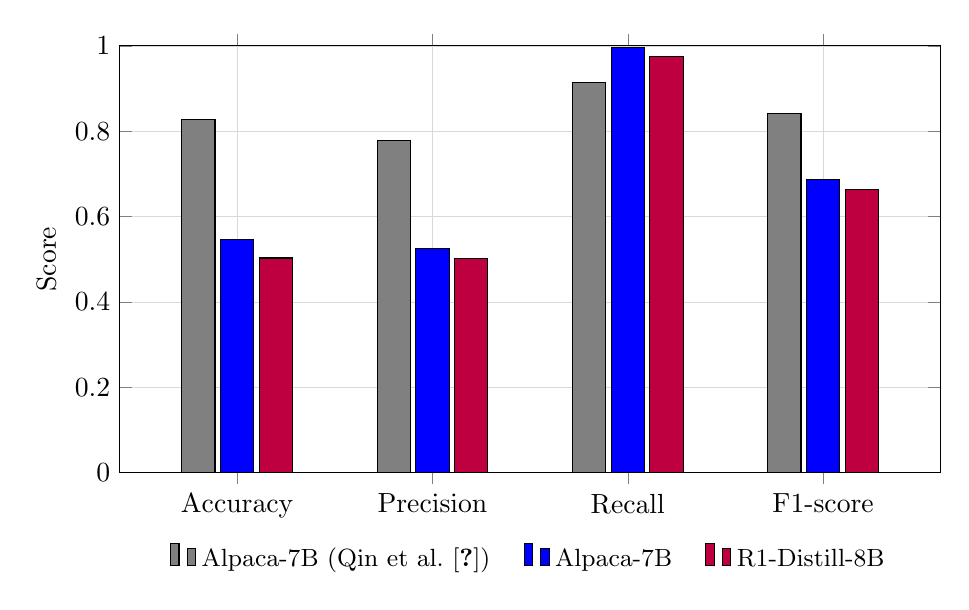
\begin{tikzpicture}
        \begin{axis}[
            ybar, bar width=12pt,
            symbolic x coords={Accuracy, Precision, Recall, F1-score},
            xtick=data, ymin=0, ymax=1,
            ylabel={Score}, width=12cm, height=7cm, grid=both,
            major grid style={line width=.2pt, draw=gray!30},
            minor grid style={draw=gray!10},
            enlarge x limits=0.2,
            legend style={
                at={(0.5,-0.15)}, anchor=north,
                /tikz/every even column/.append style={column sep=10pt},
                legend columns=3, draw=none, fill=none,
                font=\small}]

            \addplot[fill=gray]   coordinates {(Accuracy,0.8274)  (Precision,0.7791)  (Recall,0.9141)  (F1-score,0.8411)};
            \addlegendentry{\modelalpaca (Qin et al.~\cite{qin2023kopa})}

            \addplot[fill=blue] coordinates {(Accuracy,0.5465) (Precision,0.5245) (Recall,0.9962) (F1-score,0.6872)};
            \addlegendentry{\modelalpaca}

            \addplot[fill=purple]   coordinates {(Accuracy,0.5027) (Precision,0.5014) (Recall,0.9759) (F1-score,0.6625)};
            \addlegendentry{\modeldeepseek}

        \end{axis}
    \end{tikzpicture}
    \caption{Comparison of our replication of the original results from Qin et al.~\cite{qin2023kopa} using \modelalpaca, along with our additional results from \modeldeepseek, all evaluated on the CoDeX-S test set.}
    \label{fig:codex_kopa_evaluation}
\end{figure}

\begin{table}
    \centering
    \begin{tabular}{l|c|c|c|c}
        \toprule
        \textbf{Model}        & \textbf{Acc}   & \textbf{P} & \textbf{R} & \textbf{F1}    \\
        \midrule

        \modelalpaca (Theirs) & \textbf{82.74} & 77.91      & 91.41      & \textbf{84.11} \\
        \modelalpaca (Ours)   & 54.65          & 52.45      & 99.62      & 68.72          \\
        \modeldeepseek (Ours) & 50.27          & 50.14      & 97.59      & 66.25          \\

        \bottomrule
    \end{tabular}
    \caption{Results from \cref{fig:codex_kopa_evaluation} in tabular format. See \cref{tab:kicgpt_detailed_comparison} in appendix for detailled comparison.}
    \label{tab:codex_kopa_evaluation}
\end{table}


% ---------------------------------------------------------
%
% CONCLUSION
%
% ---------------------------------------------------------


\section{Conclusion and Future Work}\label{sec:conclusion-and-future-work}

In summary, we examined two approaches for KGC—KICGPT, a purely prompt-based prediction method, and KoPA, a fine-tuning-based triple classification approach.
KICGPT leverages in-context learning via structured prompts and a optimized retriever, offering a training-free alternative that can be applied directly to various Large Language Models.
KoPA, by contrast, integrates structural embeddings into the LLM's weights, through training with Knowledge Prefix Adapter, enabling more targeted triple classification by unifying textual and relational cues.

Our empirical results highlight that while prompt-based methods like KICGPT benefit from flexibility and reduced computational demands, performance and output consistency can vary depending on the chosen LLM's internal knowledge and adherence to prompt instructions.
Fine-tuning-based methods such as KoPA can be more consistent, though they often incur longer training times and may require careful balancing between textual generation and structural consistency to avoid overconfident predictions.

Overall, these findings suggest that the optimal approach to Knowledge Graph Completion hinges on task requirements and resource constraints: KICGPT excels when rapid deployment is a priority, whereas KoPA offers more robust control over the classification process at the cost of additional training.
Future research may focus on hybrid strategies that jointly leverage the prompt-driven adaptability of KICGPT and the structural grounding of KoPA. Such endeavors could address current limitations—such as handling large, incomplete, and evolving knowledge graphs in a more controlled and scalable manner—while further improving link prediction and triple classification performance.

\bibliography{main}

\appendix


\section{Detailled Results}

In \cref{tab:kicgpt_detailed_comparison}, we extend the detailed comparisons from Wei et al.~\cite{wei2023kicgpt} to include our results, and similarly, in \cref{tab:kopa_detailled_comparison}, we incorporate our findings alongside those of Qin et al.~\cite{qin2023kopa}.

\begin{table}
    \centering
    \begin{tabular}{l|l|c|c|c|c|}
        \toprule
        \textbf{Category} & \textbf{Model}                           & \textbf{MRR}      & \textbf{Hits@1}   & \textbf{Hits@3}   & \textbf{Hits@10}  \\
        \midrule

        \multirow{9}{*}{Triple-based}
        & RESCAL~\cite{nickel2011three}            & 0.467             & 0.439             & 0.478             & 0.516             \\
        & TransE~\cite{bordes2013translating}      & 0.243             & 0.043             & 0.441             & 0.532             \\
        & DistMult~\cite{yang2014embedding}        & 0.430             & 0.390             & 0.440             & 0.490             \\
        & ComplEx~\cite{trouillon2016complex}      & 0.440             & 0.410             & 0.460             & 0.510             \\
        & RotatE~\cite{sun2019rotate}              & 0.476             & 0.428             & 0.492             & 0.571             \\
        & TuckER~\cite{balavzevic2019tucker}       & 0.470             & 0.443             & 0.482             & 0.526             \\
        & HAKE~\cite{zhang2020learning}            & 0.497             & 0.452             & 0.516             & 0.582             \\
        & CompGCN~\cite{vashishth2019composition}  & 0.479             & 0.443             & 0.494             & 0.546             \\
        & HittER~\cite{chen-etal-2021-hitter}      & 0.496             & 0.449             & 0.514             & 0.586             \\
        \midrule

        \multirow{5}{*}{Text-based}
        & Pretrain-KGE~\cite{zhang2020pretrain}    & 0.235             & -                 & -                 & 0.557             \\
        & KG-BERT~\cite{yao2019kgbert}             & 0.216             & 0.041             & 0.302             & 0.524             \\
        & StAR~\cite{wang2021structure}            & 0.364             & 0.222             & 0.436             & 0.647             \\
        & MEM-KGC (w/o EP)~\cite{choi2021mem}      & 0.533             & 0.473             & 0.570             & 0.636             \\
        & MEM-KGC (w/ EP)~\cite{choi2021mem}       & \underline{0.557} & \underline{0.475} & \underline{0.604} & \textbf{0.704} \\
        \midrule

        \multirow{2}{*}{LLM-based}
        & ChatGPT$_{zero-shot}$~\cite{zhu2023llms} & -                 & 0.190             & -                 & -                 \\
        & ChatGPT$_{one-shot}$~\cite{zhu2023llms}  & -                 & 0.212             & -                 & -                 \\

        \midrule

        \multirow{4}{*}{KICGPT}
        & ChatGPT (Theirs)                         & \textbf{0.564}    & \textbf{0.478}    & \textbf{0.612}    & \underline{0.677} \\
        & Mistral-7B (Ours)                        & 0.3112            & 0.1707            & 0.3711            & 0.5862            \\
        & DeepSeek-7B (Ours)                       & 0.2700            & 0.1233            & 0.2994            & 0.6145            \\
        & DeepSeek-7B$_{zero-shot}$ (Ours)         & 0.2461            & 0.0980            & 0.2580            & 0.6120            \\

        \bottomrule
    \end{tabular}

    \caption{Comparison between various methods on WN18RR. The best result in terms of each metric is shown in \textbf{bold} and the second best is \underline{underlined}. Figure adapted from Wei et al.~\cite{wei2023kicgpt}.}
    \label{tab:kicgpt_detailed_comparison}
\end{table}


\begin{table}
    \centering
    \begin{tabular}{l|c|>{\columncolor{light-gray}}c|cc|>{\columncolor{light-gray}}c|}
        \toprule
        \textbf{Category} & \textbf{Model}                      & \textbf{Acc}      & \textbf{P} & \textbf{R} & \textbf{F1}       \\ \midrule

        \multirow{4}{*}{Embedding-based}
        & TransE~\cite{bordes2013translating} & 72.07             & 71.91      & 72.42      & 72.17             \\
        & DistMult~\cite{yang2014embedding}   & 66.79             & 69.67      & 59.46      & 64.16             \\
        & ComplEx~\cite{trouillon2016complex} & 67.64             & 67.84      & 67.06      & 67.45             \\
        & RotatE~\cite{sun2019rotate}         & 75.68             & 75.66      & 75.71      & 75.69             \\
        \midrule

        \multirow{1}{*}{PLM-based}
        & KG-BERT~\cite{yao2019kgbert}        & 77.30             & 70.96      & 92.43      & 80.28             \\
        \midrule

        \multirow{6}{*}{LLM-based Training-free}
        & Zero-shot(Alpaca)                   & 50.62             & 50.31      & 99.83      & 66.91             \\
        & Zero-shot(GPT-3.5)                  & 54.68             & 69.13      & 16.94      & 27.21             \\
        & ICL(1-shot)                         & 49.86             & 49.86      & 50.59      & 50.17             \\
        & ICL(2-shot)                         & 52.95             & 51.54      & 98.85      & 67.75             \\
        & ICL(4-shot)                         & 51.14             & 50.58      & 99.83      & 67.14             \\
        & ICL(8-shot)                         & 50.62             & 50.31      & 99.83      & 66.91             \\
        \midrule

        \multirow{4}{*}{LLM-based Fine-tuning}
        & KG-LLaMA~\cite{yao2023exploring}    & 79.43             & 78.67      & 80.74      & 79.69             \\
        & KG-Alpaca~\cite{yao2023exploring}   & 80.25             & 79.38      & 81.73      & 80.54             \\
        & Vanilla IT                          & 81.18             & 77.01      & 88.89      & 82.52             \\
        & Structure-aware IT                  & \underline{81.27} & 77.14      & 88.40      & \underline{82.58} \\
        \midrule

        \multirow{3}{*}{KoPA}
        & \modelalpaca (Theirs)               & \textbf{82.74}    & 77.91      & 91.41      & \textbf{84.11}    \\
        & \modelalpaca (Ours)                 & 54.65             & 52.45      & 99.62      & 68.72             \\
        & \modeldeepseek (Ours)               & 50.27             & 50.14      & 97.59      & 66.25             \\

        \bottomrule
    \end{tabular}
    \caption{Triple classification results on the CoDeX-S dataset. We report the accuracy (Acc), precision (P), recall (R), and F1-score (F1) for each method. The best \textbf{Acc / F1} results in baselines are marked with \underline{underline}, best result for accuracy is marked in \textbf{bold}. Figure adapted and extended from Qin et al.~\cite{qin2023kopa}.}
    \label{tab:kopa_detailled_comparison}
\end{table}

\end{document}
